%
%	Praxisbezug
%

\pagebreak
\section{NIS2 Analysis}

\onehalfspacing

\subsection{Running the CIS Benchmarks}

To examine the results of a CIS Benchmark, we will create a Kubernetes cluster on Microsoft Azure with the following versions:

\begin{itemize}
    \item Microsoft AKS v1.32
    \item CIS AKS Benchmark v1.7
    \item kube-bench v0.11.2
    \item SUSE Rancher v2.11.3
    \item Terraform v1.12
\end{itemize}

We will create the cluster with a default node pool and without hardening to get reproducible results that will be relevant for most environments:

\begin{lstlisting}[caption=Terraform Plan, frame=single, basicstyle=\ttfamily]
# AKS cluster
resource "azurerm_kubernetes_cluster" "cluster_az" {
  name                = "aks-${random_id.instance_id.hex}"
  location            = var.az-region
  resource_group_name = var.az-resource-group
  kubernetes_version  = var.k8version
  dns_prefix          = "aks-${random_id.instance_id.hex}"
  web_app_routing {
    dns_zone_ids = []
  }
  local_account_disabled = "false"
  default_node_pool {
    name       = "agent${random_id.instance_id.hex}"
    node_count = var.numnodes
    vm_size    = var.type
  }
  identity {
    type = "SystemAssigned"
  }
}            
\end{lstlisting}
This is the resulting AKS cluster that we will use for our test:

\begin{figure}[H]
\centering
\caption {AKS Cluster Dashboard}
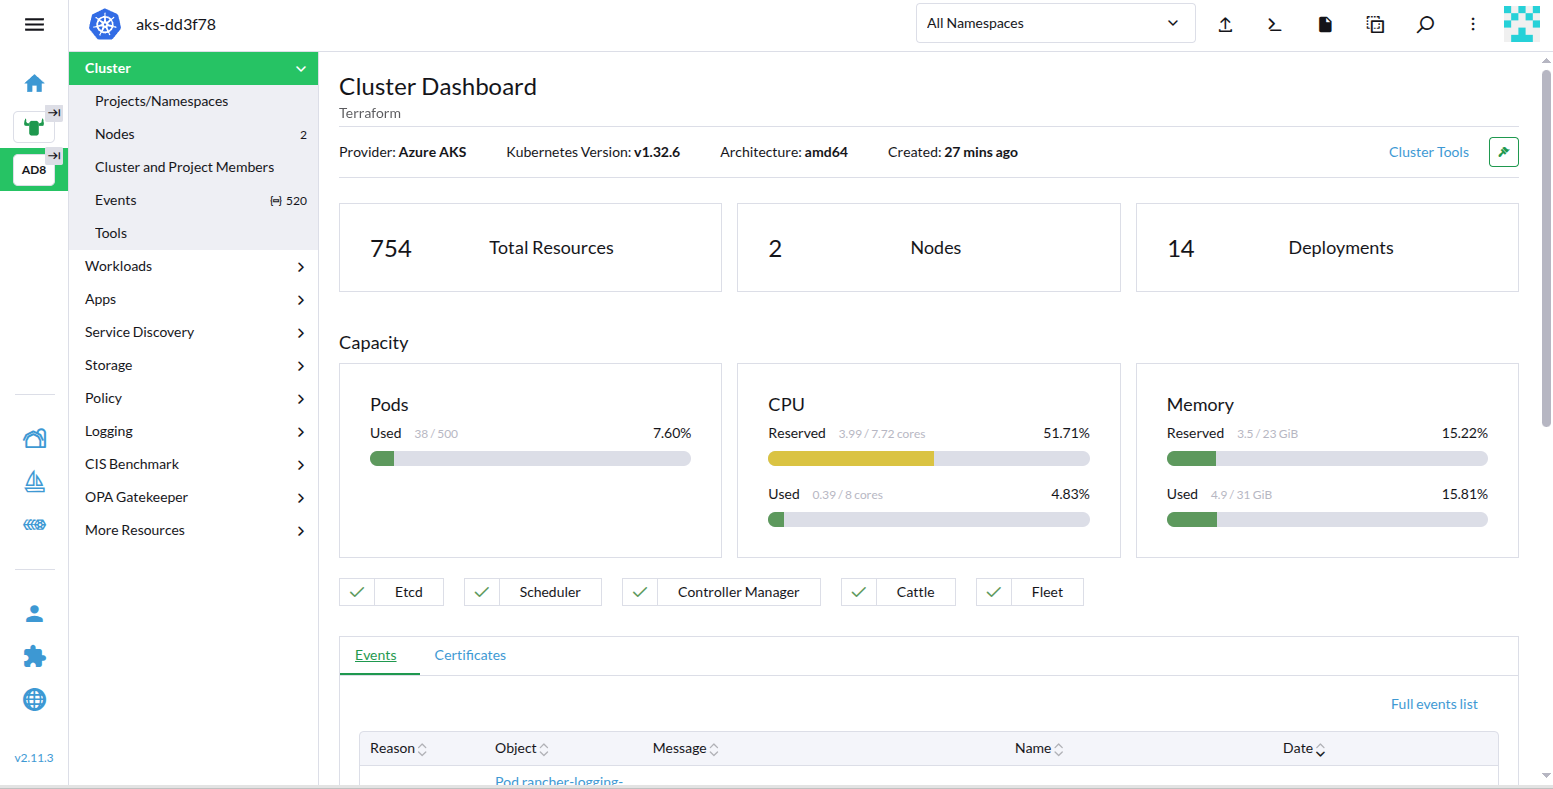
\includegraphics[width=\linewidth]{images/aks-dd3f78.png}
\label{fig:aksdd3f78}
\end{figure}

We then execute the kube-bench job as defined in Chapter 2, and the Benchmark results will become available in the job output:

\begin{figure}[H]
\centering
\caption {Kube-bench Job Output}
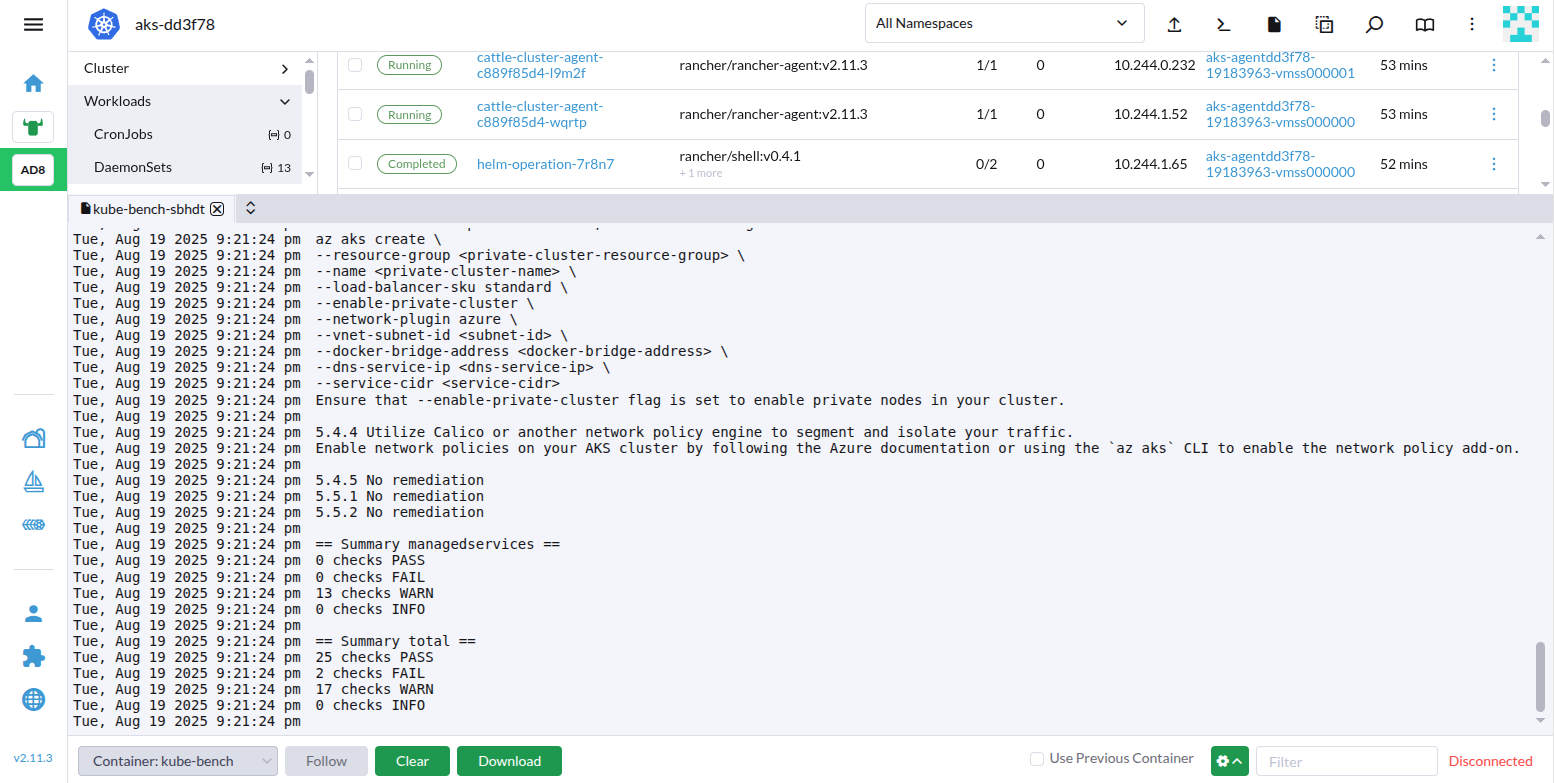
\includegraphics[width=\linewidth]{images/kube-bench-sbhdt.png}
\label{fig:kubesbhdt}
\end{figure}

\pagebreak

\subsection{Benchmarks Findings}

Let's inspect the detailed results from the CIS Benchmark scan, beginning with the worker node security:

\begin{table}[hp]
  \centering
  \caption{CIS Benchmark Scan - Worker Node}
    \begin{tabular}{| l | l | p{11cm} |}
    \hline
    State & ID & Description \\
    \hline\hline
    [PASS] & 3.1.1 & Ensure that the kubeconfig file permissions are set to 644 or more restrictive (Automated) \\
    \hline
    [PASS] & 3.1.2 & Ensure that the kubelet kubeconfig file ownership is set to root:root (Automated) \\
    \hline
    [PASS] & 3.1.3 & Ensure that the azure.json file has permissions set to 644 or more restrictive (Automated) \\
    \hline
    [PASS] & 3.1.4 & Ensure that the azure.json file ownership is set to root:root (Automated) \\
    \hline
    [PASS] & 3.2.1 & Ensure that the --anonymous-auth argument is set to false (Automated) \\
    \hline
    [PASS] & 3.2.2 & Ensure that the --authorization-mode argument is not set to AlwaysAllow (Automated) \\
    \hline
    [PASS] & 3.2.3 & Ensure that the --client-ca-file argument is set as appropriate (Automated) \\
    \hline
    [PASS] & 3.2.4 & Ensure that the --read-only-port is secured (Automated) \\
    \hline
    [PASS] & 3.2.5 & Ensure that the --streaming-connection-idle-timeout argument is not set to 0 (Automated) \\
    \hline
    [PASS] & 3.2.6 & Ensure that the --make-iptables-util-chains argument is set to true (Automated)  \\
    \hline
    [PASS] & 3.2.7 & Ensure that the --eventRecordQPS argument is set to 0 or a level which ensures appropriate event capture (Automated) \\
    \hline
    [PASS] & 3.2.8 & Ensure that the --rotate-certificates argument is not set to false (Automated) \\
    \hline
    [PASS] & 3.2.9 & Ensure that the RotateKubeletServerCertificate argument is set to true (Automated) \\
    \hline
    \end{tabular}%
  \label{tab:aksScanW}%
\end{table}%

As expected, a default installation of a Microsoft AKS cluster will pass all tests for node security, including the important CIS Benchmark test 3.2.1 for anonymous access to the Kubelet server. The CIS Benchmark documentation states the obvious for this test: "You should rely on authentication to authorize access and disallow anonymous requests."\footnote{\textit{CIS (2023)}: CIS AKS Benchmark, 3.2 Kubelet. \cite{cisAks}}

\pagebreak

Next, we'll examine the results for the policies:

\begin{table}[hp]
  \centering
  \caption{CIS Benchmark Scan - Policies}
    \begin{tabular}{| l | l | p{11cm} |}
    \hline
    State & ID & Description \\
    \hline\hline
    [FAIL] & 4.1.1 & Ensure that the cluster-admin role is only used where required (Automated) \\
    \hline
    [PASS] & 4.1.2 & Minimize access to secrets (Automated) \\
    \hline
    [PASS] & 4.1.3 & Minimize wildcard use in Roles and ClusterRoles (Automated) \\
    \hline
    [PASS] & 4.1.4 & Minimize access to create pods (Automated) \\
    \hline
    [PASS] & 4.1.5 & Ensure that default service accounts are not actively used (Automated) \\
    \hline
    [FAIL] & 4.1.6 & Ensure that Service Account Tokens are only mounted where necessary (Automated) \\
    \hline
    [PASS] & 4.2.1 & Minimize the admission of privileged containers (Automated) \\
    \hline
    [PASS] & 4.2.2 & Minimize the admission of containers wishing to share the host process ID namespace (Automated) \\
    \hline
    [PASS] & 4.2.3 & Minimize the admission of containers wishing to share the host IPC namespace (Automated) \\
    \hline
    [PASS] & 4.2.4 & Minimize the admission of containers wishing to share the host network namespace (Automated) \\
    \hline
    [PASS] & 4.2.5 & Minimize the admission of containers with allowPrivilegeEscalation (Automated) \\
    \hline
    [WARN] & 4.4.1 & Ensure latest CNI version is used (Manual) \\
    \hline
    [PASS] & 4.4.2 & Ensure that all Namespaces have Network Policies defined (Automated) \\
    \hline
    [PASS] & 4.5.1 & Prefer using secrets as files over secrets as environment variables (Automated) \\
    \hline
    [WARN] & 4.5.2 & Consider external secret storage (Manual) \\
    \hline
    [WARN] & 4.6.1 & Create administrative boundaries between resources using namespaces (Manual) \\
    \hline
    [WARN] & 4.6.2 & Apply Security Context to Your Pods and Containers (Manual) \\
    \hline
    [PASS] & 4.6.3 & The default namespace should not be used (Automated) \\
    \hline
    \end{tabular}%
  \label{tab:aksScanP}%
\end{table}%

In this section, we encounter two failures due to excessive admin access usage and four warnings concerning network and workload configuration, which should be remedied with the appropriate hardening.

\pagebreak

As the final step, we'll examine the results for managed services:

\begin{table}[hp]
  \centering
  \caption{CIS Benchmark Scan - Managed Services}
    \begin{tabular}{| l | l | p{11cm} |}
    \hline
    State & ID & Description \\
    \hline\hline
    [WARN] & 5.1.1 & Ensure Image Vulnerability Scanning using Microsoft Defender for Cloud (MDC) (Manual) \\
    \hline
    [WARN] & 5.1.2 & Minimize user access to Azure Container Registry (ACR) (Manual) \\
    \hline
    [WARN] & 5.1.3 & Minimize cluster access to read-only for Azure Container Registry (ACR) (Manual) \\
    \hline
    [WARN] & 5.1.4 & Minimize Container Registries to only those approved (Manual) \\
    \hline
    [WARN] & 5.2.1 & Prefer using dedicated AKS Service Accounts (Manual) \\
    \hline
    [WARN] & 5.3.1 & Ensure Kubernetes Secrets are encrypted (Manual) \\
    \hline
    [WARN] & 5.4.1 & Restrict Access to the Control Plane Endpoint (Manual) \\
    \hline
    [WARN] & 5.4.2 & Ensure clusters are created with Private Endpoint Enabled and Public Access Disabled (Manual) \\
    \hline
    [WARN] & 5.4.3 & Ensure clusters are created with Private Nodes (Manual) \\
    \hline
    [WARN] & 5.4.4 & Ensure Network Policy is Enabled and set as appropriate (Manual) \\
    \hline
    [WARN] & 5.4.5 & Encrypt traffic to HTTPS load balancers with TLS certificates (Manual) \\
    \hline
    [WARN] & 5.5.1 & Manage Kubernetes RBAC users with Azure AD (Manual) \\
    \hline
    [WARN] & 5.5.2 & Use Azure RBAC for Kubernetes Authorization (Manual) \\
    \hline
    \end{tabular}%
  \label{tab:aksScanM}%
\end{table}%

All tests in this section are set to warning level, as they mainly deal with systems outside of the Kubernetes cluster, such as the container registry. Also, in the remediations for this section, we can find the recommendation to move from public AKS to private AKS and private endpoints, which would significantly reduce the attack surface.

\subsection{Relevance for NIS2 Article 21}

The identified failures in the scan are both linked to the NIS2 technical implementation guidance 6.3, which generally calls for a "deny-all, permit-by-exception policy."\footnote{See \textit{ENISA (2025)}: Technical Implementation Guidance. \cite{enisaTech}}

Following the principle of least privilege is part of basic cyber hygiene. It should be standard for all critical IT systems that follow established principles for good governance.

To fully comply with the requirements of the NIS2 Directive, additional hardening measures would need to be taken for our cluster by implementing the requirements outlined in the CIS AKS Benchmark results.

\subsection{Implications for DORA compliance}

To support DORA compliance, CIS Security released in April 2025 a mapping for the CIS Controls v8.1 and DORA.\footnote{\textit{CIS (2025)}: CIS Controls v8.1 Mapping to DORA. \cite{cisMapDora}}

The mappings seem to be very similar to the mappings for the NIS2 Directive; a detailed analysis could be the subject of a further paper, with a similar outcome likely.

\subsection{Overall Compliance and Risk Mitigation}

We have seen Microsoft's Azure Kubernetes Engine partly pass the AKS CIS Benchmark v1.7 and might need additional hardening for full compliance. The other major hosted versions of Kubernetes, Google's Kubernetes Engine (GKE) and Amazon's Elastic Kubernetes Service (EKS), also offer CIS compliance and remediation guidance to their customers.

On-premise Kubernetes distributions, such as SUSE's Rancher or Red Hat's OpenShift, offer optional CIS compliance and hardening, too. 

Ensuring that an IT system, such as a Kubernetes cluster, scores a passing grade on the CIS Benchmarks supports basic cyber hygiene and should be part of any IT Security Policy.

\subsection{Outlook}

Article 21 of the NIS 2 Directive outlines the cybersecurity risk-management measures essential entities must implement to protect their networks and information systems. These measures are designed to prevent and minimize the impact of cyber incidents on both the entities and their customers. It outlines critical cybersecurity practices that every business under the NIS2 regulations must have in place. 

One mandatory cybersecurity measure under Article 21 is basic cyber hygiene practices and training, as described in paragraph 2(g).

This requirement is where NIS2, the CIS Controls, and the CIS Benchmarks intersect. The CIS Benchmarks outline and implement procedures to fulfill CIS Control 04, Secure Configuration, a crucial requirement for basic cyber hygiene and part of any IT Security Policy.

As we've seen above, CIS Benchmarks can be used to enforce good security practices by automatically checking for deviations and issues. CIS Benchmarks can also recommend the necessary steps for remediation.

We can conclude that a passing result for the appropriate CIS Benchmark can serve as a good indicator of whether the Kubernetes cluster is NIS2 compliant.

Passing the CIS Benchmark alone is not a sufficient indicator, though, as the NIS2 Directive includes many more aspects than the basic cyber hygiene outlined in Article 21; however, failing the CIS Benchmark, as in our case, will be a clear indicator that the Kubernetes cluster as part of the IT platform is not NIS2 compliant.

NIS2 is a legal framework, and compliance will be mandatory for European critical entities, ensuring widespread adoption. Unlike the CISecurity or ISO 27001 frameworks, adherence to the NIS2 Directive's requirements is not optional for entities classified as important or particularly important; it will be mandated by law.

In addition to Article 21, the NIS2 Directive also contains Article 23, which outlines the requirements for EU-wide incident reporting. Article 23 defines what constitutes an incident, the mandatory reports, and the content required in these reports. With pan-European reporting of cyber attacks, a coordinated response should become much more manageable.
